\documentclass[14pt]{extbook}
\usepackage{multicol, enumerate, enumitem, hyperref, color, soul, setspace, parskip, fancyhdr} %General Packages
\usepackage{amssymb, amsthm, amsmath, latexsym, units, mathtools} %Math Packages
\everymath{\displaystyle} %All math in Display Style
% Packages with additional options
\usepackage[headsep=0.5cm,headheight=12pt, left=1 in,right= 1 in,top= 1 in,bottom= 1 in]{geometry}
\usepackage[usenames,dvipsnames]{xcolor}
\usepackage{dashrule}  % Package to use the command below to create lines between items
\newcommand{\litem}[1]{\item#1\hspace*{-1cm}\rule{\textwidth}{0.4pt}}
\pagestyle{fancy}
\lhead{Progress Quiz 2}
\chead{}
\rhead{Version A}
\lfoot{4389-3341}
\cfoot{}
\rfoot{Summer C 2021}
\begin{document}

\begin{enumerate}
\litem{
Find the equation of the line described below. Write the linear equation in the form $ y=mx+b $ and choose the intervals that contain $m$ and $b$.\[ \text{Perpendicular to } 5 x + 4 y = 5 \text{ and passing through the point } (-4, 8). \]\begin{enumerate}[label=\Alph*.]
\item \( m \in [1.13, 1.31] \hspace*{3mm} b \in [10.92, 11.39] \)
\item \( m \in [0.28, 0.91] \hspace*{3mm} b \in [-11.74, -10.48] \)
\item \( m \in [0.28, 0.91] \hspace*{3mm} b \in [10.92, 11.39] \)
\item \( m \in [-0.85, -0.52] \hspace*{3mm} b \in [4.04, 4.84] \)
\item \( m \in [0.28, 0.91] \hspace*{3mm} b \in [11.61, 12.83] \)

\end{enumerate} }
\litem{
Solve the equation below. Then, choose the interval that contains the solution.\[ -7(-10x -16) = -19(-14x -15) \]\begin{enumerate}[label=\Alph*.]
\item \( x \in [-3.12, -1.99] \)
\item \( x \in [1.49, 2.62] \)
\item \( x \in [-1.19, -0.91] \)
\item \( x \in [-0.89, -0.78] \)
\item \( \text{There are no real solutions.} \)

\end{enumerate} }
\litem{
Solve the equation below. Then, choose the interval that contains the solution.\[ -19(-8x + 3) = -11(-2x -16) \]\begin{enumerate}[label=\Alph*.]
\item \( x \in [-0.95, -0.73] \)
\item \( x \in [1.55, 1.82] \)
\item \( x \in [0.83, 1] \)
\item \( x \in [-0.73, -0.55] \)
\item \( \text{There are no real solutions.} \)

\end{enumerate} }
\litem{
Write the equation of the line in the graph below in Standard Form $Ax+By=C$. Then, choose the intervals that contain $A, B, \text{ and } C$.
\begin{center}
    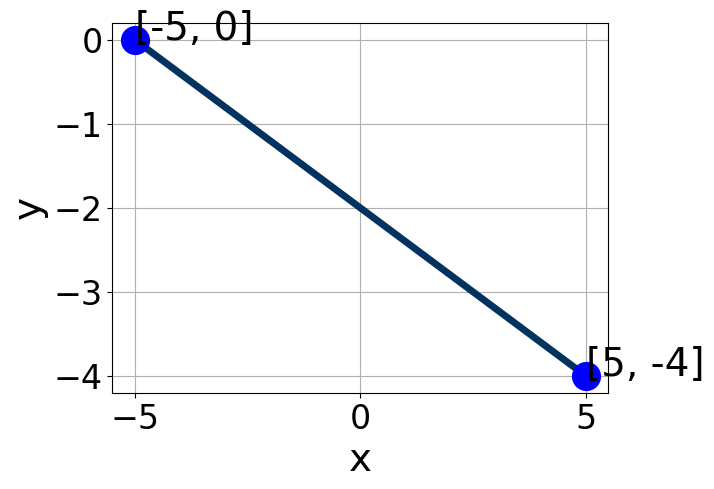
\includegraphics[width=0.5\textwidth]{../Figures/linearGraphToStandardCopyA.png}
\end{center}
\begin{enumerate}[label=\Alph*.]
\item \( A \in [-3.1, -0.3], \hspace{3mm} B \in [-7.1, -4.2], \text{ and } \hspace{3mm} C \in [8.3, 10.6] \)
\item \( A \in [-0.4, 1.1], \hspace{3mm} B \in [-2.3, -0.3], \text{ and } \hspace{3mm} C \in [0, 4.5] \)
\item \( A \in [1.6, 4.5], \hspace{3mm} B \in [3.2, 6.5], \text{ and } \hspace{3mm} C \in [-10.7, -9.3] \)
\item \( A \in [1.6, 4.5], \hspace{3mm} B \in [-7.1, -4.2], \text{ and } \hspace{3mm} C \in [8.3, 10.6] \)
\item \( A \in [-0.4, 1.1], \hspace{3mm} B \in [-0.2, 1.1], \text{ and } \hspace{3mm} C \in [-2.5, 1.1] \)

\end{enumerate} }
\litem{
Solve the linear equation below. Then, choose the interval that contains the solution.\[ \frac{8x + 5}{8} - \frac{-9x + 6}{5} = \frac{5x + 3}{2} \]\begin{enumerate}[label=\Alph*.]
\item \( x \in [11.8, 13.9] \)
\item \( x \in [-2.2, 0] \)
\item \( x \in [6.2, 7.8] \)
\item \( x \in [-0.4, 2] \)
\item \( \text{There are no real solutions.} \)

\end{enumerate} }
\litem{
Find the equation of the line described below. Write the linear equation in the form $ y=mx+b $ and choose the intervals that contain $m$ and $b$.\[ \text{Parallel to } 3 x - 5 y = 8 \text{ and passing through the point } (4, 4). \]\begin{enumerate}[label=\Alph*.]
\item \( m \in [0, 1.5] \hspace*{3mm} b \in [-0.5, 1.34] \)
\item \( m \in [1.5, 2.2] \hspace*{3mm} b \in [1.4, 2.05] \)
\item \( m \in [0, 1.5] \hspace*{3mm} b \in [1.4, 2.05] \)
\item \( m \in [-0.9, -0.2] \hspace*{3mm} b \in [6.21, 7.56] \)
\item \( m \in [0, 1.5] \hspace*{3mm} b \in [-2.12, -0.92] \)

\end{enumerate} }
\litem{
Solve the linear equation below. Then, choose the interval that contains the solution.\[ \frac{3x -9}{2} - \frac{6x + 7}{6} = \frac{-8x + 3}{7} \]\begin{enumerate}[label=\Alph*.]
\item \( x \in [1.4, 3.3] \)
\item \( x \in [0.6, 1.3] \)
\item \( x \in [2.9, 4.4] \)
\item \( x \in [11.3, 12.6] \)
\item \( \text{There are no real solutions.} \)

\end{enumerate} }
\litem{
First, find the equation of the line containing the two points below. Then, write the equation in the form $ y=mx+b $ and choose the intervals that contain $m$ and $b$.\[ (8, 3) \text{ and } (-2, -4) \]\begin{enumerate}[label=\Alph*.]
\item \( m \in [-0.48, 0.74] \hspace*{3mm} b \in [-2.85, -2.4] \)
\item \( m \in [-0.48, 0.74] \hspace*{3mm} b \in [-5.02, -4.7] \)
\item \( m \in [-0.48, 0.74] \hspace*{3mm} b \in [2.56, 3.03] \)
\item \( m \in [-0.48, 0.74] \hspace*{3mm} b \in [-2, -1.98] \)
\item \( m \in [-0.94, 0.14] \hspace*{3mm} b \in [-5.81, -5.06] \)

\end{enumerate} }
\litem{
Write the equation of the line in the graph below in Standard Form $Ax+By=C$. Then, choose the intervals that contain $A, B, \text{ and } C$.
\begin{center}
    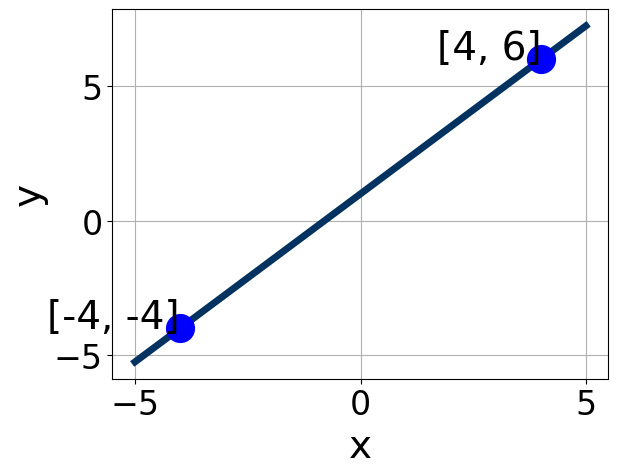
\includegraphics[width=0.5\textwidth]{../Figures/linearGraphToStandardA.png}
\end{center}
\begin{enumerate}[label=\Alph*.]
\item \( A \in [-3.25, 3.75], \hspace{3mm} B \in [-0.28, 2.73], \text{ and } \hspace{3mm} C \in [0.7, 2.5] \)
\item \( A \in [2, 9], \hspace{3mm} B \in [-4.28, -2.48], \text{ and } \hspace{3mm} C \in [-6.4, -1.6] \)
\item \( A \in [-7, -3], \hspace{3mm} B \in [2.35, 4.17], \text{ and } \hspace{3mm} C \in [3.7, 5.1] \)
\item \( A \in [-3.25, 3.75], \hspace{3mm} B \in [-2.3, -0.22], \text{ and } \hspace{3mm} C \in [-3.9, 0.4] \)
\item \( A \in [2, 9], \hspace{3mm} B \in [2.35, 4.17], \text{ and } \hspace{3mm} C \in [3.7, 5.1] \)

\end{enumerate} }
\litem{
First, find the equation of the line containing the two points below. Then, write the equation in the form $ y=mx+b $ and choose the intervals that contain $m$ and $b$.\[ (-5, 6) \text{ and } (9, 3) \]\begin{enumerate}[label=\Alph*.]
\item \( m \in [-1.7, 0.14] \hspace*{3mm} b \in [-5.04, -4.83] \)
\item \( m \in [0.16, 3.02] \hspace*{3mm} b \in [-0.09, 3.74] \)
\item \( m \in [-1.7, 0.14] \hspace*{3mm} b \in [2.8, 6.12] \)
\item \( m \in [-1.7, 0.14] \hspace*{3mm} b \in [10.9, 11.73] \)
\item \( m \in [-1.7, 0.14] \hspace*{3mm} b \in [-6.78, -5.15] \)

\end{enumerate} }
\end{enumerate}

\end{document}